%538
\newpage
\subsection{ミニサッカーゲームで遊んでみよう}



文字とかんたんな\ruby{図形}{ず|けい}を使うだけでもゲームを作ることができます。実際にできあがっているプログラムを動かして試してみましょう。

スクリプトエディタの、ファイル→「開く」メニューから「kick.hsp」を読み込みましょう。

作業は、すべて「/home/ユーザー名/04」フォルダで行ないます。

見つからない場合は、まわりの友達か、近くの先生に聞いてみてください。



[F5]キーで実行すると、ミニサッカーゲームが動きます。



\begin{figure}[H]
    \begin{center}
      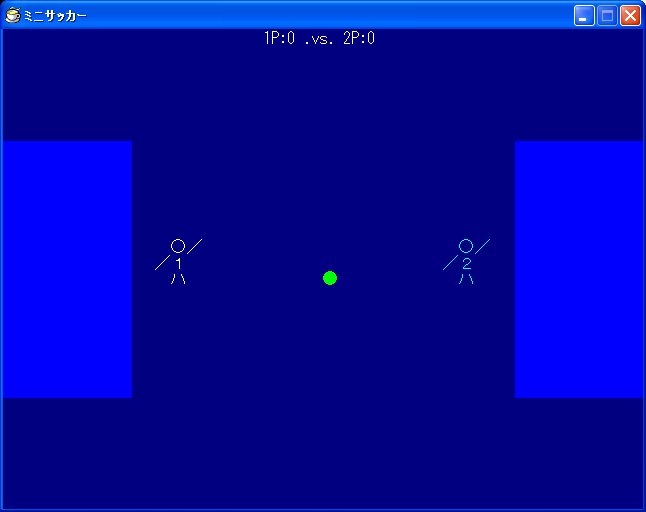
\includegraphics[keepaspectratio,width=9.075cm,height=7.197cm]{text04-img/s_kick.png}
      \caption{ミニサッカーゲームの画面}
    \end{center}
    \label{fig:prog_menu}
\end{figure}


このゲームは二人で\ruby{対戦}{たい|せん}します。

\ruby{隣}{となり}の席にいる人と、2人1組になって\ruby{一緒}{いっ|しょ}に遊んでみてください。

左側の「1」の人をキーボードの左側で\ruby{操作}{そう|さ}します。




\ \ \ \ [W]

[A] \ \ \ \ [D] \ \ \ \ [S] = ゴール前にもどる

\ \ \ \ [X]



右側の「2」の人をキーボードの右側で操作します。




\ \ \ \ [↑]

[←] \ \ \ [→] \ \ \ \ [Enter] = ゴール前にもどる

\ \ \ \ [↓]




それぞれのプレイヤーは足でボールを蹴って遠くに飛ばすことができます。

\ \ \ \ 「1」の人は右のゴールへ、

\ \ \ \ 「2」の人は左のゴールへボールを入れたら点が入ります。


\ \ \ \ 3点先に取った人の勝ちです。

\ \ \ \ 同じグループの友達と対戦してみましょう。



\begin{figure}[H]
    \begin{center}
      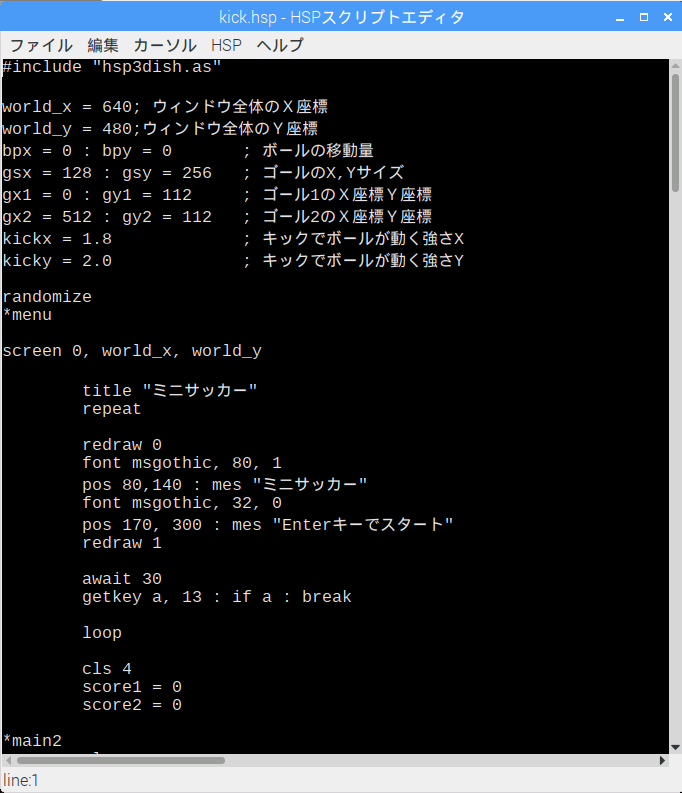
\includegraphics[keepaspectratio,width=9.657cm,height=11.229cm]{text04-img/s_kicksrc.png}
      \caption{ミニサッカーゲームのプログラム}
    \end{center}
    \label{fig:prog_menu}
\end{figure}


\newpage
\subsection{例題に挑戦しよう}

終わってしまった人は、以下の例題にも挑戦してみよう。


・ミニサッカーゲームの人を改造する

・ミニサッカーゲームのボールや色を変える

・ミニサッカーゲームの動きを改造する



例題の考え方がわからない時は、近くのTAか先生に聞いてください。

わからない所は、そのままにせず、必ず答えを見つけてから先に進みましょう。
\newpage
\subsection{例題4-1 ミニサッカーゲームの人を\ruby{改造}{かい|ぞう}する}

\begin{description}
    \item \textgt{\bf 考え方}
\end{description}

ミニサッカーゲーム(kick.hsp)のプログラムを改造してゲームの内容を変えてみましょう。

このゲームに\ruby{登場}{とう|じょう}する人は、実は文字の組み合わせで作られています。

\ruby{顔文字}{かお|も|じ}(\^{}\^{}) みたいですね。


\begin{figure}[H]
    \begin{center}
      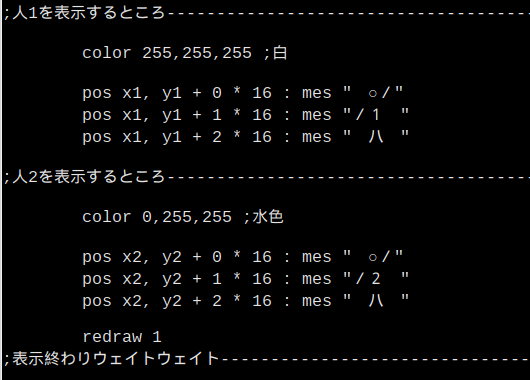
\includegraphics[keepaspectratio,width=12.326cm,height=8.123cm]{text04-img/s_kicksrc1.png}
      \caption{ミニサッカーゲームのプログラム}
    \end{center}
    \label{fig:prog_menu}
\end{figure}



プログラムから、mes命令で人を表示している部分を探して改造してみましょう。

mes命令は、

\begin{description}
    \item \textgt{\bf mes \ “文字”}
\end{description}


のように必ず「”」の記号で文字を囲む必要があるので忘れないでください。

\begin{description}
    \item \textgt{\bf 例題1 答え}
\end{description}


[F5]キーを押して改造した人がきちんと表示されるかどうか確認しましょう。

\ \ \ \ 人を改造することで、見た目が変わってあなただけのゲームに変わります。

改造ができたらTAや周りの友達にも見せてあげましょう。

\clearpage

\begin{description}
    \item \textgt{\bf [\ruby{重要}{じゅう|よう}]エラーが出て動かなくなった時は}
\end{description}

プログラムを改造していると、[F5]キーを押して実行しようとしても、エラーが\ruby{発生}{はっ|せい}して動かなくなったり、絵がおかしくなったりすることがあります。


\begin{figure}[H]
    \begin{center}
      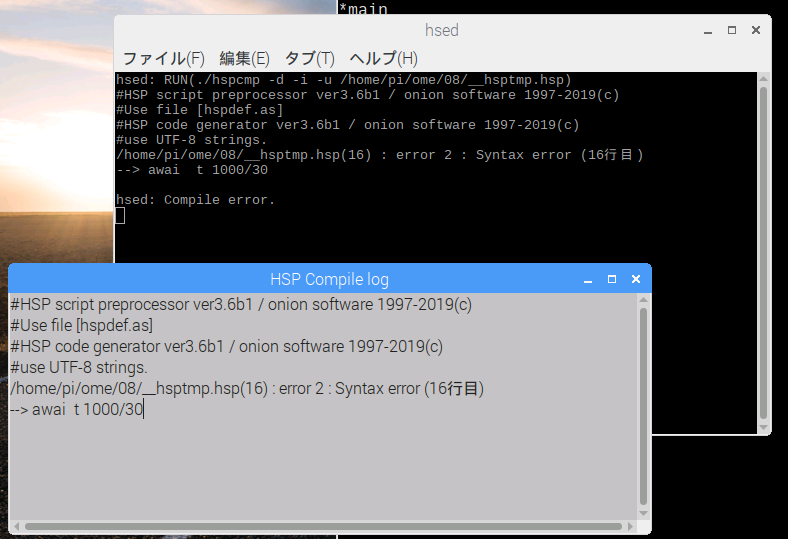
\includegraphics[keepaspectratio,width=11.324cm,height=7.756cm]{text04-img/s_hsperror.png}
      \caption{エラーの表示}
    \end{center}
    \label{fig:prog_menu}
\end{figure}

エラーが発生した時は、エラーの内容と「(xx行目)」というエラーの場所が示されます。

エディタの左下にカーソルがある行番号が表示されているので、エラーの場所を見直してください。

わからない時は、先生かTAに質問してみましょう。

どうしても動かなくなってしまった時には、元になっているファイルが保存されているので、

「/usr/local/share/ome/04」フォルダ内の元のファイル(kick.hsp)をもう一度コピーして使ってみてください。
%770
\newpage
\subsection{例題4-2 ミニサッカーゲームのボールや色を変える}

\begin{description}
    \item \textgt{\bf 考え方}
\end{description}

ミニサッカーゲーム(kick.hsp)のプログラムを改造してゲームの内容を変えてみましょう。

ゲームの中に出てくるサッカーボールもmes命令によって表示されています。


\begin{figure}[H]
    \begin{center}
      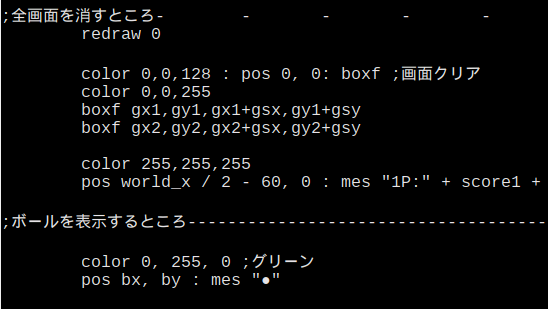
\includegraphics[keepaspectratio,width=14.499cm,height=8.123cm]{text04-img/s_kicksrc2.png}
      \caption{ミニサッカーゲームのプログラム}
    \end{center}
    \label{fig:prog_menu}
\end{figure}


このボールも変えることができます。

プログラムの中から、ボールを出している部分を探して変更しましょう。



color命令は、色を決める命令だということを覚えていますか?

第2回で覚えたcolor命令の使い方を思い出しながら、ボールの色を変えてみましょう。


\begin{figure}[H]
    \begin{center}
      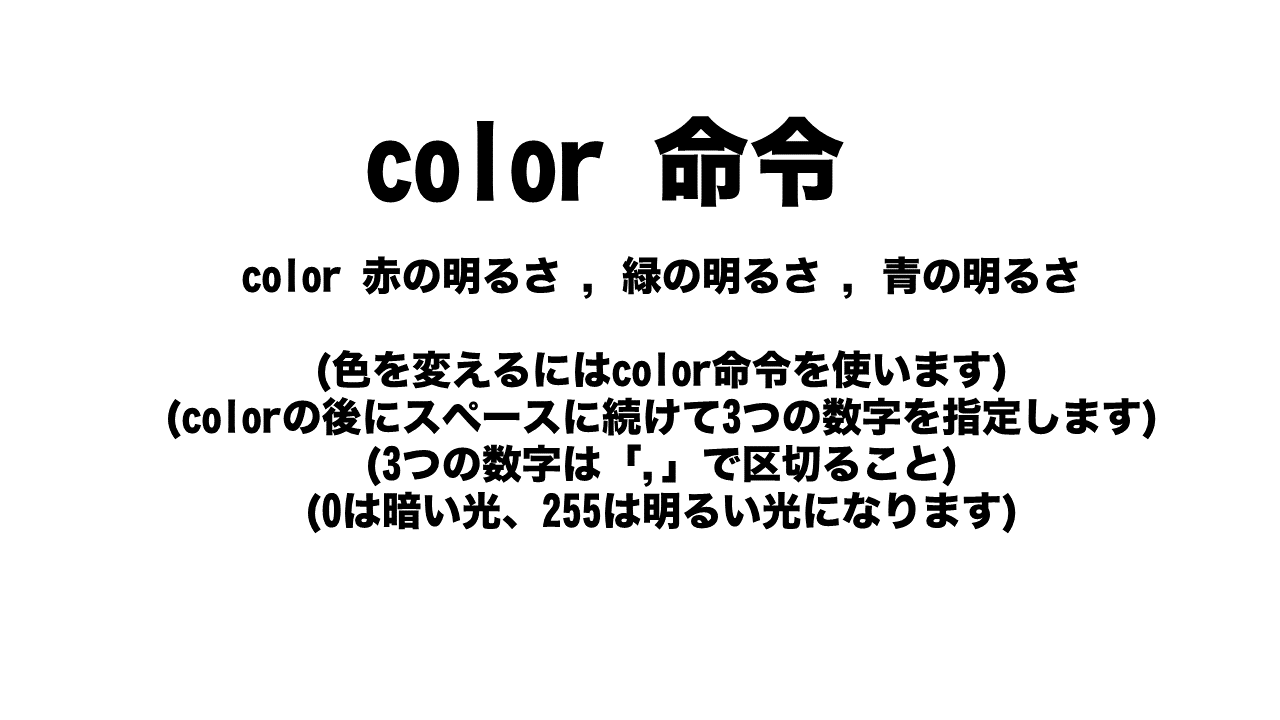
\includegraphics[keepaspectratio,width=12.409cm,height=7.62cm]{text04-img/s_kicksrc3.png}
    \end{center}
    \label{fig:prog_menu}
\end{figure}


このゲームでは画像を一切使っていません。

背景のゴール、人、ボールも含めてすべてプログラムの中で決めています。

boxf命令は、好きな大きさの\ruby{四角形}{し|かく|けい}を画面に出すことのできる命令です。

この命令とcolorを組み合わせて背景となる色やゴールを出しています。



\ruby{実際}{じっ|さい}に色を書き\ruby{換}{か}えて、オリジナルのサッカーゲームを作ってみましょう。

タイトルの文字や、得点を表示する文字も変えることができます。




\begin{description}
    \item \textgt{\bf 例題4-2 答え}
\end{description}


[F5]キーを押して改造した部分がきちんと表示されるかどうか確認しましょう。

\ \ \ \ プログラムを改造することで、見た目が変わってあなただけのゲームに変わります。

改造ができたらTAや周りの友達にも見せてあげましょう。
%861
\newpage
\subsection{例題4-3 ミニサッカーゲームの動きを改造する}

\begin{description}
    \item \textgt{\bf 考え方}
\end{description}

ミニサッカーゲーム(kick.hsp)のプログラムを改造してゲームの内容を変えてみましょう。

このプログラムでは、変数を使って人の動きや、ボールの動きを計算しています。

変数の代入と計算の方法を覚えていますか?



プログラムの最初に、変数に値を代入しています。

この値を変更することで、ゲームの動きが大きく変わります。


\begin{figure}[H]
    \begin{center}
      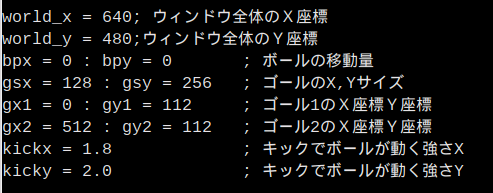
\includegraphics[keepaspectratio,width=13.044cm,height=5.106cm]{text04-img/s_kicksrc4.png}
      \caption{ミニサッカーゲームのプログラム}
    \end{center}
    \label{fig:prog_menu}
\end{figure}


でたらめに書き直してもエラーになったり、処理が遅くなったりするので、あまり大きく変えないようにしましよう。

どの変数が、どのような働きをしているかをコメントとして書いてあります。


\begin{description}
    \item \textgt{\bf \ \ 変数 = 数字 \ \ \ \ \ \ \ \ \ \ \ \ \ \ \ \ \ \ \ \ \ \ \ \ \ \ \ \ \ \ \ \ \ \ ; コメント}
\end{description}

となっている時、「; コメント」の部分は、プログラムの実行には関係ないですがメモを残す意味で、文字が書かれています。「;」記号から後ろはコメントとして扱われるルールだということを覚えておきましょう。

Xは横方向の動きを表しています。Yは縦方向です。

数字を変えてどのように変わるか試してみましょう。


\begin{description}
    \item \textgt{\bf 例題4-3 答え}
\end{description}



「kickx = 1.8」の数字を少しだけ大きくしてみましょう。

(大きくしすぎないようにしてください)

「kicky = 2.0」なども変えてみると、どうなるか確認してみましょう。



[F5]キーを押して改造したゲームがきちんと動くか確認しましょう。

改造ができたらTAや周りの友達にも見せてあげましょう。

